\section{The model}
The state of a molecular dynamics system is fully described by seven variables per atom; three positions, three velocities plus the atom type. These phase variables are evolved through the laws of motion. It is common to apply periodic boundary conditions so that $r_i = r_i + L_i$, where $L_i$ is the system length in the $i$'th dimension. Applied periodic boundary conditions in all directions implies constant volume. The atomic forces are calculated as the gradient of a chosen potential that can differ quite a lot depending on the requirements of the model. A noble gas like Argon can be modelled with a simple potential called the Lennard-Jones potential which will be discussed below. With this potential, one can calculate equilibrium thermodynamic properties that are in good agreement with experimental values \cite{verlet1967computer}. System statistics are sampled as ensable averages through ergodicity over large times. A typical Molecular Dynamics algorithm is described in figure \ref{fig:flow_simple_md}.
\begin{figure}[h]
\framebox{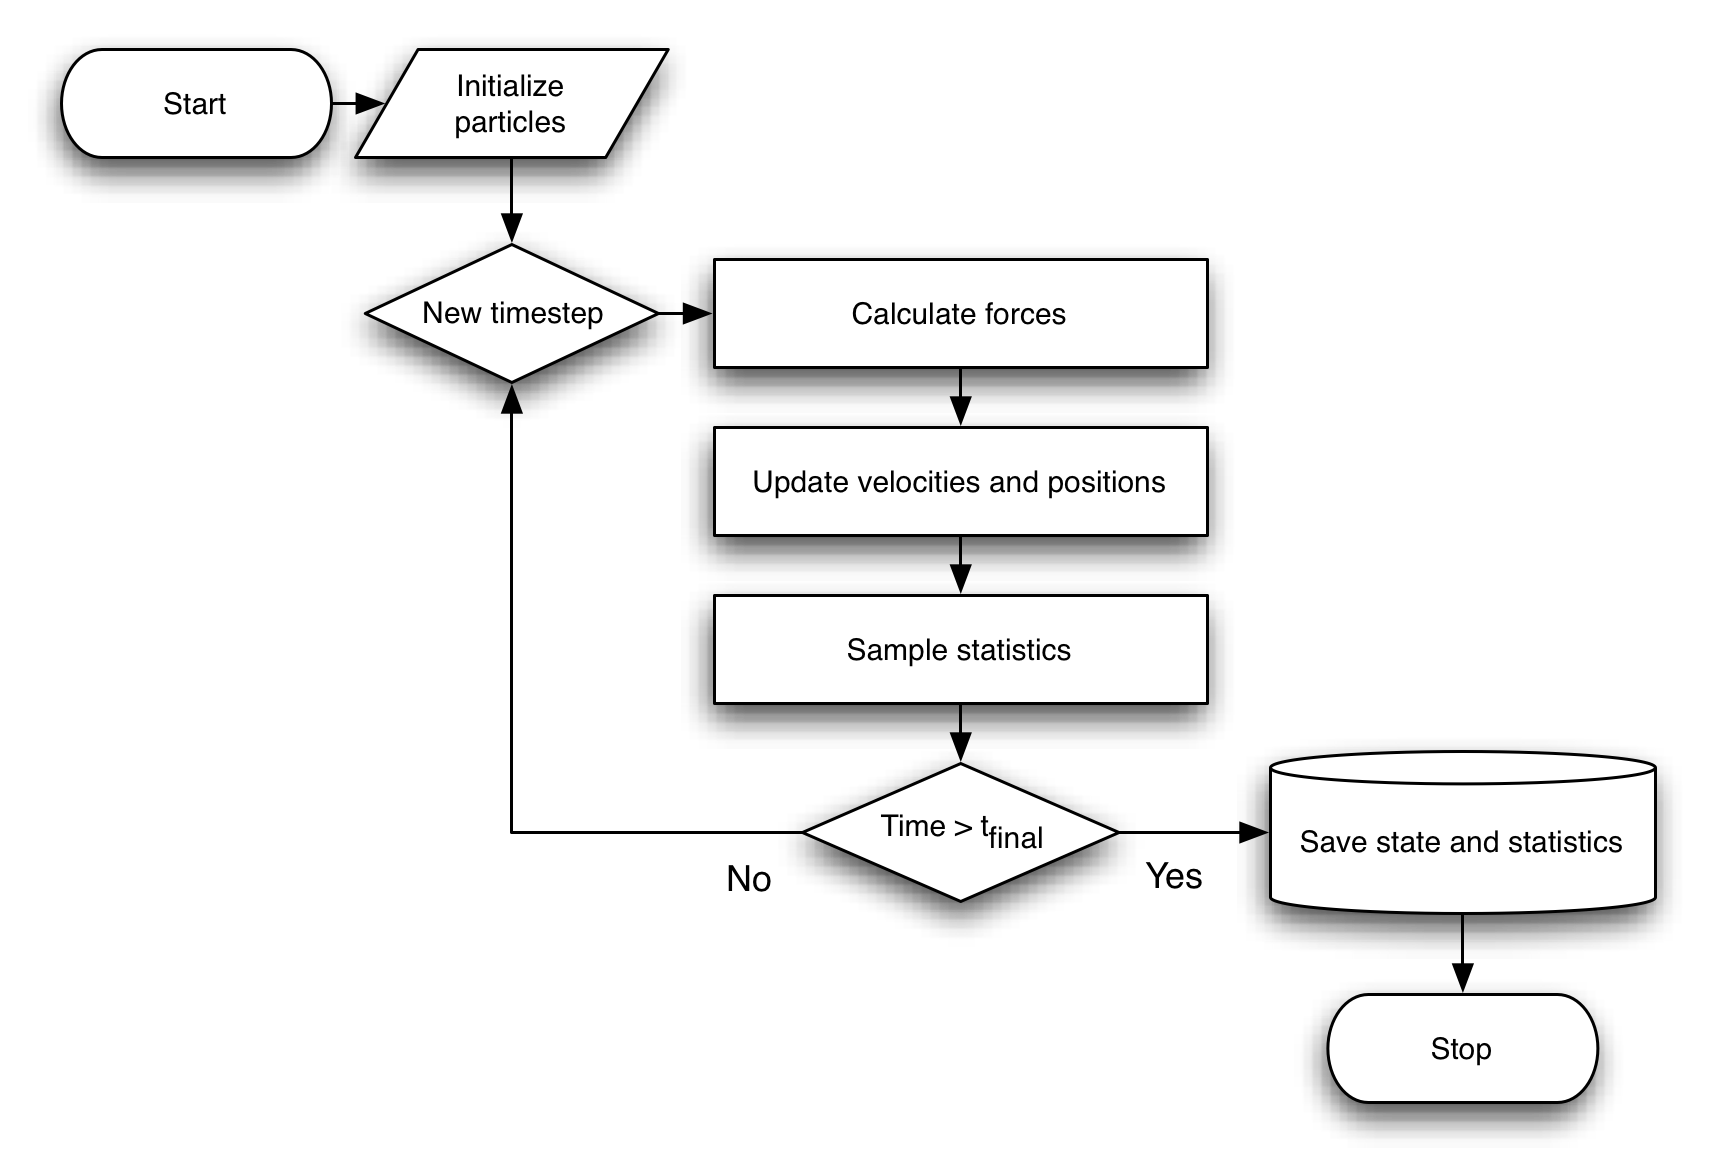
\includegraphics[width=0.5\textwidth, trim=-5cm 0cm -10cm 0cm, clip]{MD/figures/SimpleMD.png}}
\label{fig:flow_simple_md}
\centering
\caption{Flow chart illustrating how a typical Molecular Dynamics algorithm is written. }
\end{figure}
\subsection{Force calculation - potentials}
In general, the potential energy is given as a function of the configuration given by the atom positions
\begin{align}
	U(\textbf{r}) = \sum_{i<j}U_2(r_{ij}) + \sum_{i<j<k} U_r(\vec r_i, \vec r_j, \vec r_k) + ...,
\end{align}
where $\vec r$ is the phase space point, $U_n$ is a function of the positions of $n$ atoms, $r_{ij}$ is the relative distance between atom $i$ and $j$, $\vec r_i$ is the position of atom $i$. Advanced potentials like ReaxFF can even have 5-atom contributions to the energy\cite{van2001reaxff}. The reason for this is simple; when three atoms are close to each other, the electron configuration might be different than if there were only two atoms. These effects play a large role in forming molecules, such as water.\\
Numerically, the calculation of forces is the most expensive part of the whole program, so for simple systems or educationally purposes it might be sufficient to use the Lennard-Jones potential.

\subsubsection{Lennard-Jones potential}
\label{sec:md_lj_potential}
We often see this potential referred to as the 6-12 potential. It is a function that contains the two main properties of atomic forces; the short-ranged Pauli repulsion and the long-ranged van der Waals force. The potential is only between pairs of atoms
\begin{align}
	\label{eq:md_potential_energy}
	U_{LJ}(r_{ij}) = 4\epsilon\left[\left(\frac{\sigma}{r_{ij}}\right)^{12} - \left(\frac{\sigma}{r_{ij}}\right)^{6}\right],
\end{align}
where $r_{ij}$ is the relative distance between atom $i$ and $j$, $\epsilon$ and $\sigma$ are coupling constants giving the depth of the potential well and the distance where the potential is zero. We can extend this potential to behave differently for several atom types, by allowing the coupling constants to be dependent of the two interacting atoms. The Lennard-Jones potential is then written as
\begin{align}
	U_{LJ}(r_{ij}) = 4\epsilon_{AB}\left[\left(\frac{\sigma_{AB}}{r_{ij}}\right)^{12} - \left(\frac{\sigma_{AB}}{r_{ij}}\right)^{6}\right],
\end{align}
where the coupling constants are specified for interacting atom pairs of type $A$ and $B$. If the system has only two different atoms, it is usually called a \textit{binary Lennard-Jones fluid}. The force is given as the gradient of this potential yielding 
\begin{align*}
	\vec F_{LJ}(\vec{r_{ij}}) = -\nabla U_{LJ}(r_{ij}) = -24\epsilon_{AB}\left[2\left(\frac{\sigma_{AB}^{12}}{r_{ij}^{13}}\right) - \left(\frac{\sigma_{AB}^6}{r_{ij}^7}\right)\right]\vec u_{ij},
\end{align*}
where $\vec u_{ij}$ is the unit vector pointing from atom $i$ to atom $j$. In this thesis, we will only study the LJ-potential, so we simplify the notation by choosing $\vec F_{LJ} = \vec F$ and $U_{LJ} = U$.
\subsection{Time integration}
Once we know how to calculate the forces, we have everything we need to evolve the system through time. The system is integrated with Newton's laws with some integration scheme. In MD-simulations, it is common to chooce the Velocity Verlet algorithm. Time is discretized into timesteps, $\Delta t$, so the state variables and the acceleration $\vec a$ at $t=n\Delta t$ are written as
\begin{align*}
	\vec r(t) & = \vec r_n\\
	\vec v(t) & = \vec v_n\\
	\vec a(t) & = \vec a_n.
\end{align*}
Each timestep is computed as follows
\begin{enumerate}
	\item $\vec v_{n+1/2} = \vec v_{n} + \frac{1}{2}\vec a_{n}\Delta t$
	\item $\vec r_{n+1} = \vec v_{n} + \vec v_{n+1/2}\Delta t$
	\item $\vec a_{n+1} = {1\over m}\vec F(\vec r_{n+1})$
	\item $\vec v_{n+1}   = \vec v_{n+1/2} + \frac{1}{2}\vec a_{n+1}\Delta t$
\end{enumerate}
which gives a local error of order $(\Delta t)^4$ \cite{allen1989computer}. If we look carefully, we notice that step 1 and 4 can be combined to obtain the scheme that contains fewer arithmetic operations
\begin{enumerate}
	\item $\vec v_{n+1/2} = \vec v_{n-1/2} + \vec a_{n}\Delta t$
	\item $\vec r_{n+1} = \vec v_{n} + \vec v_{n+1/2}\Delta t$
	\item $\vec a_{n+1} = {1\over m}\vec F(\vec r_{n+1})$,
\end{enumerate}
where we only at the first timestep have to calculate $\vec v_{1/2}$ by following the first scheme.


